%%%%%%%%%%%%%%%%%%%%%%%%%%%%%%%%%%%%%%%%%%%%%%%%%%%%%%%%%%%%%%%%%%%%%%%%%%%%%%%%%%%%%%%%%%%%%%%%%%%%%%%%%%%%%%%%%%%%%%%%%%%%%%%%%%%%%%%%%%%%%%%%%%%%%%%%%%%
% This is just an example/guide for you to refer to when submitting manuscripts to Frontiers, it is not mandatory to use Frontiers .cls files nor frontiers.tex  %
% This will only generate the Manuscript, the final article will be typeset by Frontiers after acceptance.   
%                                              %
%                                                                                                                                                         %
% When submitting your files, remember to upload this *tex file, the pdf generated with it, the *bib file (if bibliography is not within the *tex) and all the figures.
%%%%%%%%%%%%%%%%%%%%%%%%%%%%%%%%%%%%%%%%%%%%%%%%%%%%%%%%%%%%%%%%%%%%%%%%%%%%%%%%%%%%%%%%%%%%%%%%%%%%%%%%%%%%%%%%%%%%%%%%%%%%%%%%%%%%%%%%%%%%%%%%%%%%%%%%%%%

%%% Version 3.4 Generated 2018/06/15 %%%
%%% You will need to have the following packages installed: datetime, fmtcount, etoolbox, fcprefix, which are normally inlcuded in WinEdt. %%%
%%% In http://www.ctan.org/ you can find the packages and how to install them, if necessary. %%%
%%%  NB logo1.jpg is required in the path in order to correctly compile front page header %%%

\documentclass[utf8]{frontiersSCNS} % for Science, Engineering and Humanities and Social Sciences articles
%\documentclass[utf8]{frontiersHLTH} % for Health articles
%\documentclass[utf8]{frontiersFPHY} % for Physics and Applied Mathematics and Statistics articles

%\setcitestyle{square} % for Physics and Applied Mathematics and Statistics articles
\usepackage{url,hyperref,lineno,microtype,subcaption}
\usepackage[onehalfspacing]{setspace}
\linenumbers

\usepackage{hhline}
\usepackage[first=0,last=9]{lcg}
\newcommand{\ra}{\rand0.\arabic{rand}}
\usepackage{color}
\usepackage{threeparttable}
\usepackage{pgfplots}
\pgfplotsset{compat=1.15}
\usepackage{natbib}
%\PassOptionsToPackage{dvipsnames,svgnames,table}{xcolor}
\usepackage{xcolor,colortbl}
\usepackage{amssymb}% http://ctan.org/pkg/amssymb
\usepackage{pifont}% http://ctan.org/pkg/pifont
\newcommand{\cmark}{\text{\ding{51}}}
\newcommand{\xmark}{\text{\ding{55}}}


\def\keyFont{\fontsize{8}{11}\helveticabold }
%\newcommand{\orcidauthorA}{0000-0003-2395-2883} 
%add \orcidA{} to the affiliate author
\def\firstAuthorLast{Largeron {et~al.}} %use et al only if is more than 1 author
\def\Authors{Chloé Largeron $^{1,2}$, Marie Dumont $^{1}$, Samuel Morin $^{1}$, Aaron Boone $^{2}$, Matthieu Lafaysse $^{1}$, Sammy Metref $^{3}$, and Emmanuel Cosme $^{3}$}
% Affiliations should be keyed to the author's name with superscript numbers and be listed as follows: Laboratory, Institute, Department, Organization, City, State abbreviation (USA, Canada, Australia), and Country (without detailed address information such as city zip codes or street names).
% If one of the authors has a change of address, list the new address below the correspondence details using a superscript symbol and use the same symbol to indicate the author in the author list.
\def\Address{$^{1}$Univ. Grenoble Alpes, Université de Toulouse, Météo-France, CNRS, CNRM, Centre d'Études de la Neige, Grenoble, France\\
	$^{2}$CNRM, Université de Toulouse, Météo-France, CNRS, Toulouse, France\\
	$^{3}$Universit\'e Grenoble Alpes, CNRS, IRD, IGE, Grenoble, France}
% The Corresponding Author should be marked with an asterisk
% Provide the exact contact address (this time including street name and city zip code) and email of the corresponding author
\def\corrAuthor{Chloé Largeron}

\def\corrEmail{chloe.largeron@gmail.com}





\begin{document}

\onecolumn
\firstpage{1}

\title[A review of data assimilation applied to snow hydrology in mountain regions]{A review of data assimilation applied to snow hydrology in mountain regions} 

\author[\firstAuthorLast ]{\Authors} %This field will be automatically populated
\address{} %This field will be automatically populated
\correspondance{} %This field will be automatically populated
\extraAuth{}% If there are more than 1 corresponding author, comment this line and uncomment the next one.
%\extraAuth{corresponding Author2 \\ Laboratory X2, Institute X2, Department X2, Organization X2, Street X2, City X2 , State XX2 (only USA, Canada and Australia), Zip Code2, X2 Country X2, email2@uni2.edu}


\maketitle


\begin{abstract}

	\section{}
Snow on the ground is a key component for land surface hydrology, especially in mountain areas where it governs the amount and timing of water availability in downstream areas. Snow is involved in relevant climate feedbacks and contributes to natural hazards such as avalanches and floods. The monitoring and forecasting of snow properties is thus required. The estimation of water equivalent of snow cover (SWE) is crucial for hydrological applications, where SWE can be indirectly measured by satellite. The accuracy of SWE estimations depends also on the study area, that are more challenging in mountain areas due to their complex topography. This study describes \textit{in situ} and remote sensing tools for measuring snow on the ground and highlights the associated limits and uncertainties of each observational technique. A description of the different degrees of complexity of snow models with their related uncertainties are given. It reviews current state-of-the-art methodologies used to optimally combine satellite measurements with snow models, through data assimilation in order to reduce the model and observation errors. The chosen data assimilation method varies with the numerical complexity of snow models as well as the availability and the type of observations. This review describes the issues and challenges associated to snow data assimilation, providing recommendations for future monitoring and prediction systems for snow hydrology in mountainous regions.
	
	
	\small
	\keyFont{ \section{Keywords:} Snow hydrology, Mountain hydrology, In-situ observations, Remote sensing, Water Equivalent of Snow cover, Data assimilation, Snow models} %All article types: you may provide up to 8 keywords; at least 5 are mandatory.
\end{abstract}



\section{Introduction}

%Parag sur climat:
%Snow on the ground is an important component of the climate system, which drastically modifies the exchange of mass, momentum and energy between the soil and atmosphere \citep{Groisman_1994,Qu_2006,Flanner_2011}. It plays a particular role in the Earth system through its unique thermal and optical properties. The presence of snow on the ground also changes the surface albedo and the aerodynamic roughness thereby impacting the energy exchange with the atmosphere \citep{Hansen_2004,Flanner_2006,Qu_2014,Hall_2006}. The low thermal conductivity of snow makes it a particularly insulating Earth surface medium, with major implications for the underlying ground temperature and permafrost. At the regional and local scales, snow on the ground plays a major role in the hydrological cycle. The influence of snow and the freeze/thaw cycles on the surface energy and water balance makes their representation in models essential for predicting the thermal characteristics and the hydrological cycle \citep{Gouttevin_2012}. 
 
Snow on the ground plays a major role in the hydrological cycle, especially in mountain areas. Seasonal snow cover is the primary water source for human use and ecosystems in mountain regions and represents up to 95 $\%$ of the water supply \citep{Liniger_1998}. In these regions, the runoff is heavily dependent on snowmelt amount and timing \citep{Bales_2006,Bowling_2003}. Monitoring of snow cover mass, most often referred to as the water equivalent of snow cover or SWE, is particularly important for water resource management with major implications for predicting natural hazards (namely avalanches and snowmelt-induced floods) \citep{Sui_2001,Finger_2012,Viviroli_2011,Freudiger_2014}. Due to the influence of snow on the surface energy and water balance \citep{Hansen_2004,Flanner_2006,Qu_2014,Hall_2006}, their representation in models are essential for predicting the thermal characteristics and the hydrological cycle \citep{Gouttevin_2012}. 

%in situ
The monitoring of the evolution of snowpack (\textit{i.e.} snow depth, density profile) and their surface properties (\textit{i.e.} albedo, surface temperature) is possible through \textit{in situ} \citep{Essery_2013,Lejeune_2018,Menard_2019} and satellite-based observations \citep{DeLannoy_2012,Dietz_2012,Gascoin_2015}. \textit{In situ} datasets are essential for the understanding of snow physical processes, and for the evaluation of snow model and satellite products \citep{Vionnet_2012,Krinner_2018}. However, point measurements inherently constrain the total number and spatial extent of data thus limiting information on the spatial heterogeneity. To monitor the evolution of the snow cover over large areas, the use of satellite observations are needed. Satellite sensors have different measurement wavelengths and employ various operating principles (active or passive). For instance, multi-spectral images from optical sensors provide information on the visible and near infra-red domain with a spatial resolution ranging from 50 cm to 500 m. Under cloud-free conditions, these images provide snow cover extent information, but also information on albedo and light absorbing particles, as well as snow microstructure \citep{Hall_1995,Hall_2007,Dietz_2012,Gascoin_2015}. Passive microwave can provide information over all atmospheric conditions at coarse resolution \citep{DeLannoy_2012}.

%Observations of snow cover areas that are particularly valuable in mountain regions have shown an improved performance of hydrological models \cite{Lee_2005,Immerzeel_2009,Finger_2015}.

%Conventional passive microwave measurements have the ability to detect through clouds and during the night. However, the  spatial resolution of around 25 km is too coarse to allow suitable measurements of snow distribution in complex snow terrain, such as mountainous regions \cite{Foster_2005,Cordisco_2006,Tedesco_2010,Li_2014}. Active microwave satellites (radar) emit a microwave signal and then measure the backscattered energy. Their high spatial resolution (spanning from a few meters to a few tens of meters) is attractive for monitoring snow in complex terrain, but the radar signal contains information that is only indirectly related to the snow conditions, and affected by other land surface elements (vegetation, topography etc.) \cite{DeLannoy_2012,Conde_2019}.

%Representation dans les modèles
The representation of snow on the ground in land surface models is crucial in view of its role in energy exchanges on the climate system and the hydrological cycle. Snow was first included into land surface models (LSMs) to obtain improved time varying estimations of the surface energy balance over cold regions \citep{Loth_1993,Lynch_1994,Douville_1995,Yang_1998,Slater_1998}. In order to better represent and account for the interactions between snow and the climate system, more complex representations of the physical properties of the snow have been progressively incorporated into LSMs \citep{Boone_2001,Dutra_2010,Decharme_2016}. %,Vionnet_2012,Wang_2013}. 
%Depending on the application, models include different levels of complexity of the snowpack, from single layer models to multi-layer schemes including snow microstructure such as Crocus \citep{Vionnet_2012}.

%combiner obs et modèles
Observations and numerical simulations represent two sources of information that can be exploited simultaneously, but inherently carry uncertainties. Data assimilation proceeds through the optimal combination of observed and simulated snow properties. This technique can be used to improve initial conditions of the snowpack for operational numerical weather prediction (NWP) or hydrological prediction \citep{Brasnett_1999,Lehning_1999,Barret_2003,Drusch_2004}. In data assimilation, observations are used to correct a set of parameters or a physical state given by a model in order to improve the overall representation of a particular system \citep{Andreadis_2006,Clark_2006,Leisenring_2011,Nagler_2008,Liu_2013}. Various data assimilation methods exist, each characterised by numerical advantages and difficulties. 

This paper aims %to provide optimal data assimilation methods for 
to review the data assimilation methods used for
snow hydrology applications in mountainous regions and provide recommendations for future monitoring adn prediction system. This paper describes (1) the different types of snow observations and their uncertainties spanning from in-situ methods to optical and microwave satellites, (2) the different complexity of snow evolution models, where the choice of the complexity of a model depends on the required applications, and  (3) different data assimilation methodologies, including a description of the limits of each method for snow applications. %, where a state of the art is given by application. 


\section{Observations}


This section describes the different observations commonly used to determine the evolution of the snow cover, emphasising on water equivalent of snow cover because of its critical relevance to mountain snow hydrology. Both advantages, disadvantages and uncertainties will be described for each type of observation. 

\subsection{\textit{In situ} observations}
%Parler des mesures automatiques manuelles. Donner techniques du SWE.
Site measurements describe the characteristics of the snow cover at a given location at one point (fixed instruments) or over an area using techniques such as terrestrial laser scanning (\textit{i.e.} camera, terrestrial laserscan). \textit{In situ} measurements are performed manually or automatically by fixed measuring instruments which provide continuous data. \textit{In situ} observations are performed either at conventional operational meteorological stations or at dedicated experimental snow sites.%, which is crucial to the understanding of the evolution of the snow cover.

\subsubsection{Meteorological stations}
Weather stations provide continuous meteorological information at a particular location, such as wind speed, temperature, incoming radiation, specific humidity and precipitation rate. Several types of stations, such as WMO synoptic stations, can also provide snow measurements for variables such as snow cover fraction (visually estimated), snow density (measured with a snow tube) and snow depth (manual or ultrasonic sensor). Manual and automatic snow measurements present in weather stations over the Europe are listed in detail in the European Snow Booklet (ESB) \citep{Haberkorn_2019}. Such weather stations cover the whole globe with a wide degree of spatial heterogeneity. For instance, Russian weather stations are generally more scarce than European and North American weather stations \citep{Ripper_2015snowpex}.

%The studies of \citet{Ripper_2015snowpex} highlight a high density of weather stations in Europe and North America, while Russian weather stations are generally more scarce.  


\subsubsection{Experimental snow sites}

The monitoring of the snowpack at conventional weather stations is often insufficient to improve process understanding and to perform a thorough snow model evaluation. To overcome this lack of information, experimental snow sites have been installed and include instruments specific for snow measurements. These sites contain automatic instruments providing daily and hourly measurements of meteorological and snow variables such as presence of snow, snow depth, SWE, snow density, albedo, snow surface temperature and runoff \citep{Pirazzini_2018}. Discontinuous measurements are often performed seasonally, especially during winter, \textit{e.g.} snow stratigraphy profile \citep{Morin_2012}. The latter is determined following the International Classification for Seasonal Snow on the Ground (ICSSG)  \citep{Fierz_2009}. Only a few experimental study snow sites measure most of the meteorological and snow variables required to determine the surface energy balance in the presence of snow. Such experimental snow sites are particularly relevant for studying the detailed evolution of the snow \citep[e.g.][]{Morin_2012,Essery_2016, Lejeune_2018}. These sites have been used extensively for snow model evaluation \citep{Magnusson_2015,Decharme_2016,Wang_2013,Piazzi_2018} and model-intercomparison, such as ESM-SnowMIP \citep{Krinner_2018}. An overview of the observation dataset at ten experimental snow sites is provided in \citet{Menard_2019}. 



%Finally, recent studies during the WMO Solid Precipitation Intercomparison Experiment (SPICE) have evaluated the performance of automated snow on the ground sensors (\textit{e.g.} snow depth, SWE) from several snow sites over the world \citep{Smith_2017,Nitu_2018}. This study has shown that most of the deviation of SWE and snow depth measurements between sensors can be attributed to the spatial variability of the snowpack. 


%Other experimental sites can be used for specific purpose as the largely exposed to strong wind experimental site of the Col du Lac Blanc (2720 m alt.) in the French Alps, which is perfectly suitable to study and measure blowing snow events \citep{Vionnet_2013,Guyomarch_2018}. 

%COST snow obs DA: \cite{Helmert_2018} 

\subsubsection{Methods of SWE measurements}
Various methods can be used to measure SWE, automatically and manually as reviewed in detail in the WMO guide to meteorological instruments and methods of observations \citep{wmo2018}. SWE manual measurements are based on bulk density samples made with a snow sampling tube (a more detailed description is given by \citet{Leppanen_2016}). The relatively sparse nature (in space and time) of manual measurements has lead to the use of more automated-type measurements. The most commonly used technique for continuous SWE measurements is the snow pillow \citep{Serreze_1999,Smith_2017}, where the pressure sensors measure the hydrostatic pressure of the snow \citep{Beaumont_1965}. Gamma-ray sensors can also be used to measure SWE continuously. Originally, these sensors used a radiation source \citep{Harding_1986}. However, for safety and environmental reasons, this instrument has been gradually replaced by natural emitted radiation such as cosmic-ray sensors and passive gamma radiation (Potassium and Thallium) sensors \citep{Choquette_2008,Martin_2008}. Cosmic-ray sensors uses harmless naturally occurring cosmic-rays to directly estimate SWE \citep{Kodama_1979}. An assessment of the different SWE measurements was detailed during the WMO SPICE experiment \citep{Smith_2017}. Recent efforts have been made to detail various snow variables and measurements methods \citep{Pirazzini_2018,Haberkorn_2019}. The uncertainties of each method are described in the following section.


\subsubsection{Measurement uncertainties}

The uncertainties associated with \textit{in situ} datasets is not only due to the intrinsic uncertainty of snow measurements. In mountain environments, the large spatial variability of snow depth around a given observation point requires that this point scale data is used with great caution \citep{Grunewald_2013}. In the studies of \citet{Lafaysse_2017} and \citet{Lejeune_2018} on snow depth measurements, the instrumental error was determined to be low (about 1 cm) compared to the spatial variability of snow depth of the surrounding environment (up to 20 cm). Conversely, the instrumental uncertainty of SWE measurements can be of the same order of magnitude than their spatial variability \citep{Smith_2017,Lafaysse_2017,Lejeune_2018, Nitu_2018}. 

SWE measurements uncertainties also vary as a function of the type of instruments. For example, snow tube measurements have been compared to layer integrated snow pit measurements and errors correspond to an average underestimation of 7.1 $\%$ \citep{Sturm_2010}. Snow pillow SWE measurements contain uncertainties which range from 6-12 $\%$ in optimal conditions (\textit{i.e.} absence of liquid water). This method is particularly suitable in cold climates. The uncertainty of snow pillow measurements increases with the presence of liquid water in the snowpack, therefore they tend to be particularly unsuitable during the snowmelt season \citep{Smith_2017,Engeset_2000}. The best SWE measurements are obtained by cosmic-ray sensors, where the accuracy is around 5-10 $\%$ \citep{Gottardi_2013}. Passive gamma radiation method has shown r$^{2}$ values higher than 0.90 compared to manual measurements for Finnish and Canadian sites \citep{Smith_2017}, where the comparison between automated and manual sensors were carried out over a distance ranging from 5 to 25 m. The difference observed between the measurements can partly be explained by the spatial variability \citep{Lejeune_2018,Smith_2017}. %The SWE sample uncertainties estimated between 5-10 $\%$ also has to be taken into account. 


%complementarity satellite and in situ

%%%%%%%%%%%%%%%%%%%%%%%%%%%%%%%%%%%%%%%%
%%%%           Satellites           %%%%

\subsection{Satellite remote sensing observations}

Remote sensing observations are crucial for monitoring the snow cover evolution over large areas. A wide variety of satellite sensors exists with various spatial resolutions composed by different categories of wavelengths. The choice of remote sensing techniques for snow products varies with the desired temporal and spatial resolution. This section describes the different types of satellite sensors (optical and microwave satellite sensors) used for monitoring snow hydrology and, indirectly, SWE. Examples of space-borne instruments or satellites used in related snow studies with their general properties classified by type of satellites sensors are summarised in Table \ref{tab:satellites}. Note than an overview of existing satellite snow products over Europe and Northern Hemisphere is available in \citet{Bartsch_2018}. 




\subsubsection{Optical sensors} 

%\paragraph{Monoscopic optical satellites}


Optical sensors use a multi-spectral imaging system in the visible and infrared domain. By design, data is only available during daytime and under cloud-free conditions. The spatial resolution of optical satellites varies from 50 cm to 1 km. Optical satellites measurements are useful for providing observations of the surface area covered by snow. They are mainly used to monitor the Snow Cover Area (SCA) providing a binary information on the presence or absence of snow per pixel, and the Snow Cover Fraction (SCF), which provides the percentage of snow coverage per pixel. This latter calculation is mostly based on two different methods. The first is the spectral unmixing method, where the total reflectance in a pixel corresponds to the sum of the reflectances due to snow, rock and vegetation \citep[e.g.][]{Painter_2009,Sirguey_2009}. Another method to produce an SCA map is based on the Normalized Difference Snow Index (NDSI) \citep{Dozier_1989, Hall_1995}, which uses reflectance data from both visible (vis) and short wave infrared (swir), thereby taking advantage of the high contrast in reflectance between the two wavelengths. In mountainous regions, snow mapping by optical satellites is affected by errors induced by the complex terrain \citep{Masson_2018}.  

Since the snow reflectance varies significantly depending on the wavelength and the structure of the snow, optical satellites are sensitive to snow impurities and snow microstructure in the visible and infrared range, however direct SWE estimations are not possible without assimilation of snow products \citep{Mary_2013}. Optical satellite data are largely used to retrieve snow cover fraction and also snow albedo covering the entire Earth at a near daily frequency, for example based on MODIS products \citep{Klein_2002} distributed trhough the National Snow and Ice Data Center. It should be noted that the use of these images remains challenging owing to difficulties in interpreting snow properties or extent in forest, complex terrain and shaded areas \citep{Rittger_2013}.


%\begin{equation}
%NDSI=\dfrac{\rho_{vis}-\rho_{swir}}{\rho_{vis}+\rho_{swir}}
%\label{ndsi}
%\end{equation}

%\paragraph{Stereoscopic optical satellites}

Stereoscopic satellites (\textit{e.g.} Pleiades 1a/1b and SPOT5/6/7) cover a specific region with different view angles with a very high resolution (VHR, 50 cm-2 m), and the acquisition of such images is generally upon request only. These images can be used for 3D mapping by photogrammetry, thereby providing topographic information. Tri-stereoscopic satellites, such as Pleiades, have been used to retrieve snow depth over an open alpine catchment by comparing snow-covered (\textit{i.e.} winter) and snow-free images \citep{Marti_2016}. Note that there remains a substantial uncertainty of the estimates of the final snow volume at the watershed scale. The snow depth measurement uncertainty is estimated to be on the order of 50 cm \citep{Marti_2016}. In addition, the calculation of snow depth leads to even larger uncertainties over steep slopes \citep{Deems_2006}. The remote sensing Lidar technology for in situ, unmanned aerial vehicles, planes or satellites (\textit{e.g.} Ice Sat, Ice Sat 2) can also be used for high resolution snow depth mapping using differences in aquired data between snow-free and snow-covered dates \citep{kwok2008, deems2013}.

The optical satellites most often used to detect snow are presented in Fig. \ref{sat} as a function of their revisit time vs. their spatial resolution.  High resolution satellites used for snow cover mapping (SPOT 6/7, Sentinel 2, Landsat 8, Pleiades 1A and 1B, see \citealp[e.g.][]{Gascoin_2019} for data access) are limited by the revisit time. In the case of SPOT 6/7 and Pleiades, the acquisition of satellite images is performed on demand, and can be superseded by higher priority requests. Monoscopic optical satellite data with most frequent revisit times are currently MODIS, PROBA-V, Sentinel 3 (S3) and VIIRS. Higher revisit times also increase the probability of obtaining cloud-free images. 


\begin{figure}
	\centering
	%	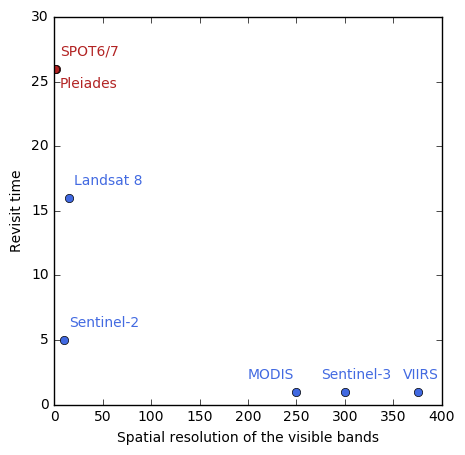
\includegraphics[scale=0.72]{Figures/sat}
	%Fig Optical satellites:

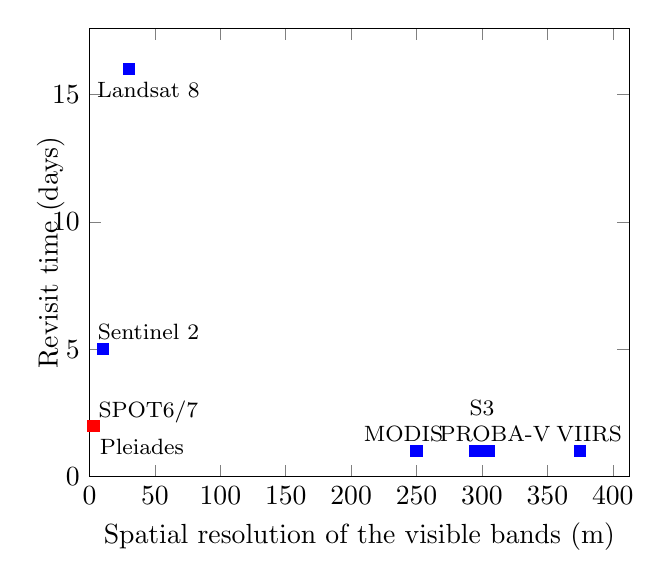
\begin{tikzpicture} 
	\begin{axis}[% 
		%coords={(xy): \thisrow{label}},%
		ylabel style={yshift=-0.4cm}, %shifting the y line text
	%	ylabel shift = 40 pt,
		ymin = 0,
		xmin=0, 
		xlabel={Spatial resolution of the visible bands (m)}, 
		ylabel={Revisit time (days)},
		xtick={0,50,100,150,200,250,300,350,400},
		ytick={0,5,10,15,20},
		scatter/classes={%
		b={mark=square*,blue},%
		r={mark=square*,red}}]
%	set(y, 'Units', 'Normalized', 'Position', [-2, 0.5, 2]);
		\addplot[scatter,only marks,%
		scatter src=explicit symbolic,
		point meta=explicit symbolic]%
		table[meta=label] {
    %    table[meta index=2]
			x y label 
			250 1 b  
			295 1 b
			305 1 b
			375 1 b
			3   2 r
			3   2 r
			30  16 b
			10  5 b
			};
	%	\node at (axis cs:0,0)

		\node [above] at (axis cs:  45,  14.5) {\footnotesize Landsat 8};
		\node [above] at (axis cs:  45,  1.7)  {\footnotesize SPOT6/7};
		\node [above] at (axis cs:  40,  0.5)  {\footnotesize Pleiades};
		\node [above] at (axis cs:  45,  5)    {\footnotesize Sentinel 2};
		\node [above] at (axis cs:  240,  1)   {\footnotesize MODIS};
		\node [above] at (axis cs:  300,  2)   {\footnotesize S3};
		\node [above] at (axis cs:  310,  1)   {\footnotesize PROBA-V};		
		\node [above] at (axis cs:  382,  1)   {\footnotesize VIIRS};
	\end{axis}
\end{tikzpicture}

%\begin{tikzpicture} 
%	\begin{axis}[% 
%	scatter/classes={% 
%		a={mark=square*,blue},% 
%		b={mark=square*,red},% 
%	}]
%%		xlabel={Spatial resolution of the visible bands (m)}, 
%%		ylabel={Revisit time (days)}]
%	\addplot[scatter,only marks,% 
%	scatter src=explicit symbolic]% 
%	table[meta=label] {
%	x y label
%	0.1 0.15 a 
%	0.85 0.52 b 
%	0.76 0.5 b 
%	0.55 0.32 c
%	}; 
%	\end{axis} 
%\end{tikzpicture}		
	\caption{Representation of optical satellite revisit time (days) vs. the corresponding spatial resolution of the visible bands (m).}\label{sat}
\end{figure}

% Stereoscopic optical satellites provide high spatial resolution images (1 m) with different angles of view allowing to get 3D images by photogrammetry. However, stereoscopic satellites cannot do daily records and have limited revisit time or available acquisitions images. The estimation of snow depth with optical satellite can be made by comparison between snow and snow-free period but with a high uncertainty \citep{Marti_2016}. These satellite can not directly measures SWE estimations.
%In summary, optical satellites are largely used to produce snow cover maps with a wide range of resolution and revisit time. Satellite sensors with the highest spatial resolution (1 m), such as Pleiades and SPOT 6/7, have a limited available images (25 days cycle). Conversely, the highest frequency satellites (daily), such as MODIS, have a coarser spatial resolution (250-500 m).

\begin{table}
	\small
	\centering
	\begin{center}
		\definecolor{grey}{gray}{0.95}
		\definecolor{LightCyan}{rgb}{0.88,1,1}
		\newcolumntype{a}{>{\columncolor{grey}}c}
		\newcolumntype{b}{>{\columncolor{white}}c}
		\begin{tabular}{ c a b a b }
			\text{} & \multicolumn{4}{c}{\textcolor{red}{\textbf{Types of satellites}}} \rule[1pt]{0pt}{10pt}\\
			\arrayrulecolor{red}\hhline{~----}
			\text{} & \textbf{Monoscopic optical}& \textbf{Stereoscopic optical} & \textbf{Passive microwave} &  \textbf{Active microwave} \rule[0pt]{0pt}{14pt}\\
			\text{} & \multicolumn{4}{c}{\textcolor{red}{\textbf{Examples of space mission}}} \rule[1pt]{0pt}{10pt}\\
			%	\arrayrulecolor{red}\hline
			\arrayrulecolor{red}\hhline{~----}
			\text{} &  \text{MODIS}& \text{SPOT-6/7} & \text{SSM/I} &  \text{ALOS 2}\rule[0pt]{0pt}{14pt}\\
			\text{} & \text{Landsat-8}& \text{Pleiades 1a/1b} & \text{SMMR} &  \text{Sentinel 1} \rule[0pt]{0pt}{10pt}\\
			\text{} & \text{Sentinel-2/3}& \text{WorldView 1-4} & \text{AMSR-E} &  \text{RADARSAT-2}\rule[0pt]{0pt}{10pt}\\
			\text{} & \text{Meteosat 8-11}& \text{} & \text{AMSU-A/B} &  \text{TerraSAR-X}\rule[0pt]{0pt}{10pt}\\	
			\text{} & \text{GOES-16-17}& \text{} & \text{} &  \text{}\rule[0pt]{0pt}{10pt}\\			
			\text{} & \text{VIIRS}& \text{} & \text{} &  \text{}\rule[0pt]{0pt}{10pt}\\
			\text{} &\text{ICESat-2}& \text{} & \text{} &  \text{}\rule[0pt]{0pt}{10pt}\\
			
			\text{} & \multicolumn{4}{c}{\textcolor{red}{\textbf{Properties}}} \rule[0pt]{0pt}{0pt}\\
			%\multicolumn{5}{c}{\textcolor{red}{\textbf{Spatial Resolution (SR), Temporal Resolution (TR), Estimations (E) and Limitations (L)}}} \rule[1pt]{0pt}{10pt}\\
			%\arrayrulecolor{red}\hline
			\arrayrulecolor{red}\hhline{~----}
			\rowcolor{LightCyan}
			\text{Spatial Res.} & \text{High (10-100 m)}& \text{Very High (1 m)} & \text{Coarse (20 km)} &  \text{Very High (1-20 m)}\rule[0pt]{0pt}{14pt}\\
			%\arrayrulecolor{black}\hline
			\text{Temporal Res.} & \text{High (daily)}& \text{On request} & \text{High (daily)} &  \text{High (daily)}\rule[0pt]{0pt}{10pt}\\
			%\arrayrulecolor{black}\hline
			\rowcolor{LightCyan}
			\text{Limits} &\text{Day/no cloud}& \text{Day/no cloud} & \text{Coarse res.} &  \text{Geometrical distorsion}\rule[0pt]{0pt}{10pt}\\
			%\arrayrulecolor{black}\hline
			\text{Retrieve data} &\text{SCF/SCE/Albedo}& \text{SD} & \text{SD/SWE} &  \text{SD/Snow wetness}\rule[0pt]{0pt}{10pt}\\
			\text{} &\text{No direct SWE}& \text{No direct SWE} & \text{SWE with T$_{b}$} &  \text{No direct SWE up to now}\rule[0pt]{0pt}{10pt}\\
			%	\text{} &\text{}& \text{} & \text{} &  \text{up to now}\rule[0pt]{0pt}{-2pt}\\
			%	\arrayrulecolor{black}\hline
			%\hline						
		\end{tabular}	
		\begin{tablenotes}
			\small
			\vspace{0.2 cm}
			MODIS, Moderate-Resolution Imaging Spectroradiometer - GOES, Geostationary Operational Environmental Satellites - VIIRS, Visible Infrared Imaging Radiometer Suite - SPOT, \textit{Satellite Pour l'Observation de la Terre} - SSM/I, Special Sensor Microwave Imager - SMMR, Scanning Multichannel Microwave Radiometer - AMSR-E, Advanced Microwave Scanning Radiometer for EOS - AMSU-A/B Advanced Microwave Sounding Unit-A/B - ALOS, Advanced Land Observing Satellite-2 - SCF, Snow Cover Fraction - SCE, Snow Cover Extent - SD, Snow Depth
		\end{tablenotes}
	\end{center}
	\caption{List of satellite data used in snow hydrology studies and their related properties classified by satellite category.}
	\label{tab:satellites}	
\end{table}

Thermal infrared satellites have also proven to be useful to monitor the evolution of the surface temperature of snow and ice covered surface \citep[e.g.][]{Dozier_2004,Freville_2014}, but the spatial resolution of the thermal bands is often too coarse for mountain regions. A recently demonstrated by \citet{Colombo_2019} monitoring the daily amplitude of snow surface temperature at high resolution from space could be extremely informative for SWE prediction. 

\subsubsection{Passive microwave}

Passive microwave sensors (10$^{-3}$ to 1 m wavelength) have the advantage of providing data under all atmospheric conditions and during day and night-time. The spectral luminance energy measured by passive microwave sensors can be utilized to calculate brightness temperature which, in turn, can be used to estimate snow depth \citep{Chang_1982}. The estimation of SWE is based on the brightness temperature alone or it can be combined with snow depth and snow density \textit{in situ} measurements \citep{Chang_1987,Cho_2017,Davenport_2012} or spatially distributed model estimates \citep{Boone_2006,Smith_2018}.

Passive microwave satellites have proven to be useful for monitoring snow cover at global and regional scales \citep{Armstrong_1995}. These satellites are used to observe the surface and can be used for surface melting observations \citep{Picard_2006} and produce a map of areas with melting snow. Studies during the GLOBSNOW project have used a combination of passive microwave and meteorological stations to produce daily SWE maps \citep{Luojus_2014}. The response of each sensor band to snow properties has been detailed by \citet{Rango_1993}. The passive microwave measurement of SWE is associated with uncertainty which is mainly caused by the vegetation cover, the unaccounted impact of snow microstructure (\textit{e.g.} density, layering, snow grain size) and errors related to the brightness temperature calibration \citep{Foster_2005}. 

The coarse spatial resolution of passive microwave sensors (around 25 km) does not permit the representation of fine scale processes, thus limiting the applicability of this method for mountainous areas. More recent satellites (\textit{e.g.} AMSR-E, AMSU-A, and AMSU-B) present a finer spatial resolution and a larger swath width allowing a better coverage efficiency. Due to the high spatial variability of the snowpack over mountain regions, passive microwave sensors measurements are often inadequate. The characteristics of passive microwave satellites used in snow studies is summarised by \citet{Konig_2001}.


%These measurements are often used to estimate snow depth and snow water equivalent. %However, the measurement of SWE requires to know the conditions of the snowpack. 
%The errors associated to the passive microwave measurement of SWE are mainly caused by the vegetation cover, the unaccounted impact of snow microstructure (density, layering, snow grain size) and errors related to the brightness temperature calibration. \citet{Foster_2005} have shown, in north America, that the error of SWE estimate due to grain size range from 9-18 mm\,w.e. (kg\,m$^{-2}$), the vegetation-induced error is generally low (3 kg\,m$^{-2}$) except in the tundra (up to 18 kg\,m$^{-2}$) and the brightness temperature error range from 6-15 kg\,m$^{-2}$. The maximum errors approached 24 kg\,m$^{-2}$.


%In order to reduce the uncertainties, different methods exist to combine microwave measurement with \textit{in situ} and/or optical measurements (see section \ref{section_DA}). 

%In summary, passive microwave satellite has the advantage to provide data under all atmospheric conditions, during daytime and nighttime. However, the coarser resolution restrain this method for complex mountainous areas. The estimation of SWE is based on the brightness temperature alone or combined with snow density measurements. Studies use a combination of \textit{in situ}, optical and microwave measurements and model to reduce SWE estimations uncertainties. SWE products uncertainties are related to observations uncertainties, which are considered to be error-free in the direct insertion method (see section \ref{section_DA}) \citep{Fletcher_2012}. In this study, snow depth was underestimated by a factor of 5 for some stations although accumulation and melt is consistent. These types of satellites detect surface melting and can easily be used to produce melting snow map.


\subsubsection{Active microwave}


Active microwave radar (RAdio Detection And Ranging) contains its own source of radiation. The detection of the scattered signal emitted by the active radar provides information on surface structure in terms of the snow roughness and microstructure. Like passive microwave, radars are not disturbed by cloud cover and can record during the day and night. Radar allows the determination of the structural properties of snowpack layers. It has been used for the retrieval of snow wetness, snow depth and SWE estimations \citep{Schmid_2014}. The radar signal is sensitive to the presence of liquid water, leading to higher backscatter for wet snow conditions \citep{Magagi_2003}. 

The very high resolution imaging (up to 1 m) is obtained with active imaging Synthetic-aperture radar sensors (SAR) that are suitable for dry and wet snow depending on their frequency and can be used to monitor the snowpack during the snowmelt period. Several studies have used SAR imaging system for the production of snowmelt maps  \citep{Shi_1994,Eckerstorfer_2016}. Recent studies have attempted to use Sentinel-1 C-band radar measurements to map snow depth and SWE at high spatial and temporal resolution \citep{Lievens_2018}. The backscatter signal of the SAR sensors allows the estimation of the snow depth, but some snow property information (such as liquid water content) must be known beforehand. A comparison of the different characteristics of SAR sensors is also given by \citet{Konig_2001}. The high spatial and temporal resolution of SAR sensors makes their use potentially well adapted for snow hydrological applications \citep{Bernier_1998,Nagler_2000,Leinss_2014,Rondeau_2016}. However, the oblique geometry viewing of SAR systems enhance geometric distortions which makes it particularly difficult to interpret in mountainous regions \citep{Veyssiere_2019}. 


%The high temporal and spatial resolution of SAR, even in cloudy condition, makes their application perfectly suitable for avalanche risk studies \citep{Caduff_2015}. 




\section{Snow modelling}

%ML:Ajouter une phrase qui décrit le role de la neige sur les modèles couplés:
Snow on the ground is a critical component within land surface models, driving major changes to the energy and mass balance computations at the surface-atmosphere interface in coupled models (climate and NWP). The representation of physical processes of snow in models is also essential for monitoring and predicting the evolution of the snowpack. A large variety of snow models exist with various representations of snow physical processes with different degrees of complexity. Snow model applications are multiple and address a wide range of needs spanning from water resource management to climate change impact studies. The complexity of a snow model varies from the most simple degree-day snow scheme (often used for hydrological applications) to multi-layer snow evolution models, which can even include explicit representations of snow microstructure (\textit{e. g.} for avalanche hazards forecasting). The physical processes represented in the different snow models complexity are shown in Fig. \ref{Fig:Model_complexity}. This section describes the different levels of complexity of snow models used in the scientific community with their corresponding applications, limits and uncertainties.


\subsection{Degree-day models}

Snow degree-day models are the simplest category of snow model for which no-explicit internal processes are represented, and the direct effects of solar radiation are neglected. Snow degree-day models are used to calculate snow mass evolution from temperature and precipitation. This method is reliable for computing snowmelt depth from daily to seasonal periods where and when temperature is a sufficient proxy of the surface energy balance \citep{Rango_1995}. %Temperature is meant to be a good indicator as the incident infrared radiation and sensible heat fluxes dominate the energy balance \citep{Ohmura_2001}.

This approach has been used for more than 100 years \citep{Clyde_1931,Collins_1934} and is still used nowadays \citep{Tobin_2013,Riboust_2019}. It is mainly used for snowmelt runoff forecast, especially for mountain basins and for studies of surface mass balance of valley glaciers \citep{Finsterwalder_1887,Singh_2000,Braithwaite_2008,Reveillet_2017}. Snow degree-day models are limited to these applications with little transferability in time and space due to the required calibration. Furthermore, degree-day models do not enable the representation of snow-atmosphere feedbacks thus limiting their accuracy for climate projections.  


\subsection{Surface energy balance models}

Surface energy balance (SEB) models incorporate a more detailed representation of the exchange of mass and energy by calculating radiative, latent, sensible and advective heat exchanges at the air/snow interface. SEB models are able to estimate snow accumulation and snowmelt, including the rate of snowmelt from hourly to seasonal time scales, through a full or partial surface energy balance computation. They were first incorporated into LSM and hydrological models, with a positive impact on discharge modelling in mountainous regions \citep{Boone_2001}. SEB models are physically-based models with a wide range of complexity. These models may include processes such as snow accumulation, snow melt, compaction, albedo variations, surface temperature evolution, sublimation and sometimes also liquid water retention and refreezing processes \citep{Tarboton_1996,Mahat_2012}. The internal physical processes of snow are described according to a single or a multi-layer snow scheme. These two categories are detailed below.


\subsubsection{Bulk/Single-layer snow models}

Single-layer snow models were used in the first versions of representations of snow in LSMs, and in some cases they are still being used, for example in operational meteorological forecasts, \textit{e.g.} the snow scheme of the \textit{European Centre for Medium range Weather Forecasting} (ECMWF) Integrated Forecast System (IFS) \citep{Dutra_2010}. Most crucially for such applications, the physical properties controlling the energy balance such as albedo, roughness, thermal properties, and turbulent fluxes, are represented. The snowpack was first represented as a composite snow-soil layer \citep{Pitman_1991,Douville_1995,Yang_1997}. In contrast to the explicit single layer schemes, the surface energy in a composite snow-soil layer model combines the soil, vegetation and snow energy balances for representing vegetation-soil-snow-atmosphere interactions. It must be emphasised that the representation of these interactions contains high uncertainties, which remain challenging to evaluate, especially when the calculation use the empirical snow fractional cover parameterisation \citep{Boone_2017,Rutter_2009}. In recent years, the increase in computer performance has led to the incorporation of more physically-based snow processes and a separate snow energy balance of snow within LSMs, the so-called explicit single-layer model, which integrates a separate surface energy balance for snow interactions with the atmosphere. 

Explicit single layer models explicitly compute the snow surface temperature, albedo, snow density, snow depth and SWE evolution with time but internal processes (especially those being depth-dependent) are not considered. Since snow is represented by a single layer, snow density is considered constant for the whole snowpack \citep{Chalita_1994,Gouttevin_2012} and can be defined as a function of the age of the snowpack, where the density increases with time \citep{Douville_1995}. Single-layer snow schemes have been specifically used in snow hydrology, NWP and climate applications \citep{Dutra_2012,Lehning_2006}. 


\subsubsection{Multi-layer snow models}\label{multilayer}

The continuous scientific progress and the increase of computer performance has led to the development of detailed snow models representing the different layers of the snowpack. Multi-layer snowpack models are also represented by different levels of complexity and vary from two layers \citep{Kondo_1990,Loth_1993,Sun_1999,Marks_1999,Yang_2003,Wang_2013,Ekici_2014} to a Lagrangian multi-layer model for which the layering evolving in time \citep{Brun_1992}. In order to obtain a good representation of the heat fluxes between the atmosphere and the snow, such models impose a higher vertical resolution for the layers at the interface \citep{Lynch_1994,Boone_2001,Decharme_2016}. Each layer of snow is characterised by state variables (snow density, snow thickness, temperature, and liquid water content, the latter two which can also be represented by the enthalpy or the energy required to melt the snowpack), allowing the calculation of the vertical gradient of temperature and density over a fine vertical resolution. A list of the physical processes and state variables integrated into multi-layer snow models is given in the Fig. \ref{Fig:Model_complexity}. Detailed multi-layer snow models incorporate heat conduction as well as more detailed physical snow processes such as snow compaction and percolation. The most complex snow models include additional internal snow processes (snow metamorphism) such as in Crocus, SNTHERM and SNOWPACK \citep{Brun_1989,Jordan_1991,Lehning_1999}. %SNTHERM: snow thermal model
In these models, the internal microstructure of snow layers and its time evolution is represented and expressed by state variables such as specific surface area and sphericity \citep{Lehning_2002,Carmagnola_2014}, enabling amonh others the representation of many complex snow-climate feedbacks. 



%Deja dit dans intercomparison model section:
%Detailed multi-layer snow scheme often hold the best performance \citep{Krinner_2018}.

\begin{figure}
	\centering
	%	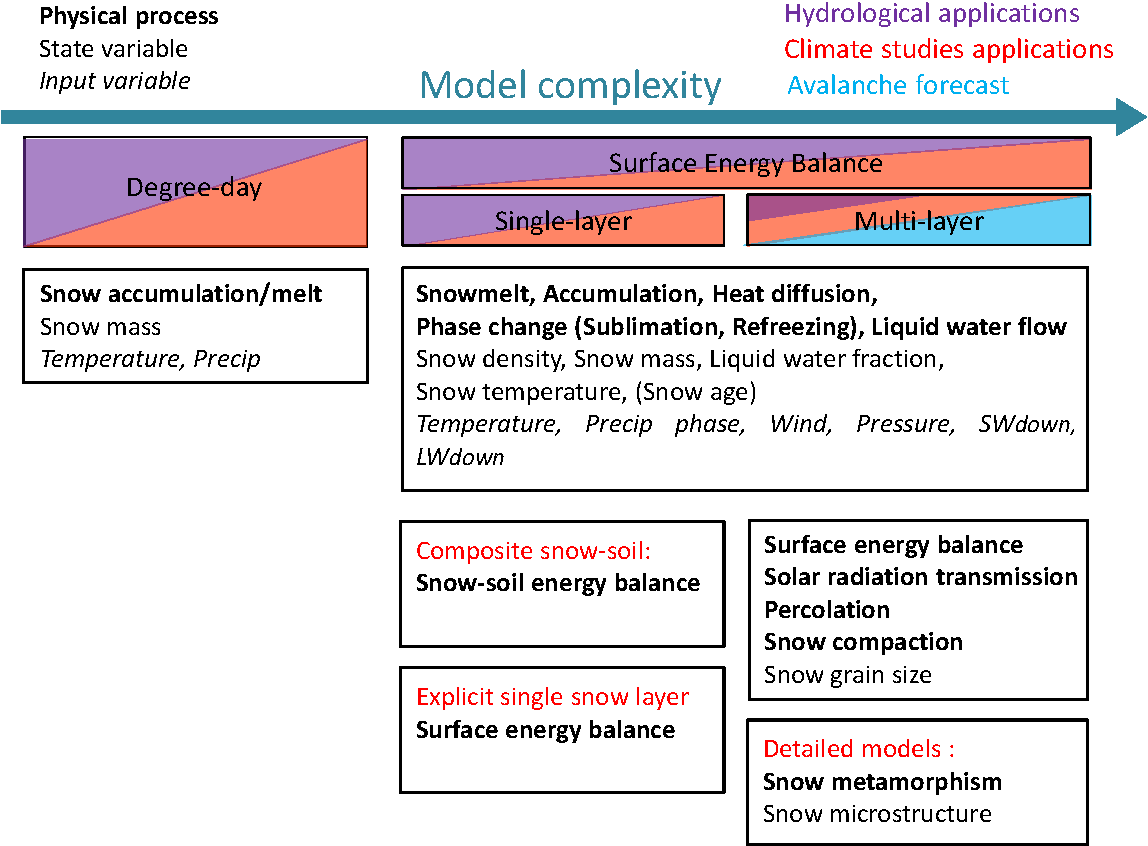
\includegraphics[scale=0.65]{Figures/Fig_modelcomplexity_AB}
	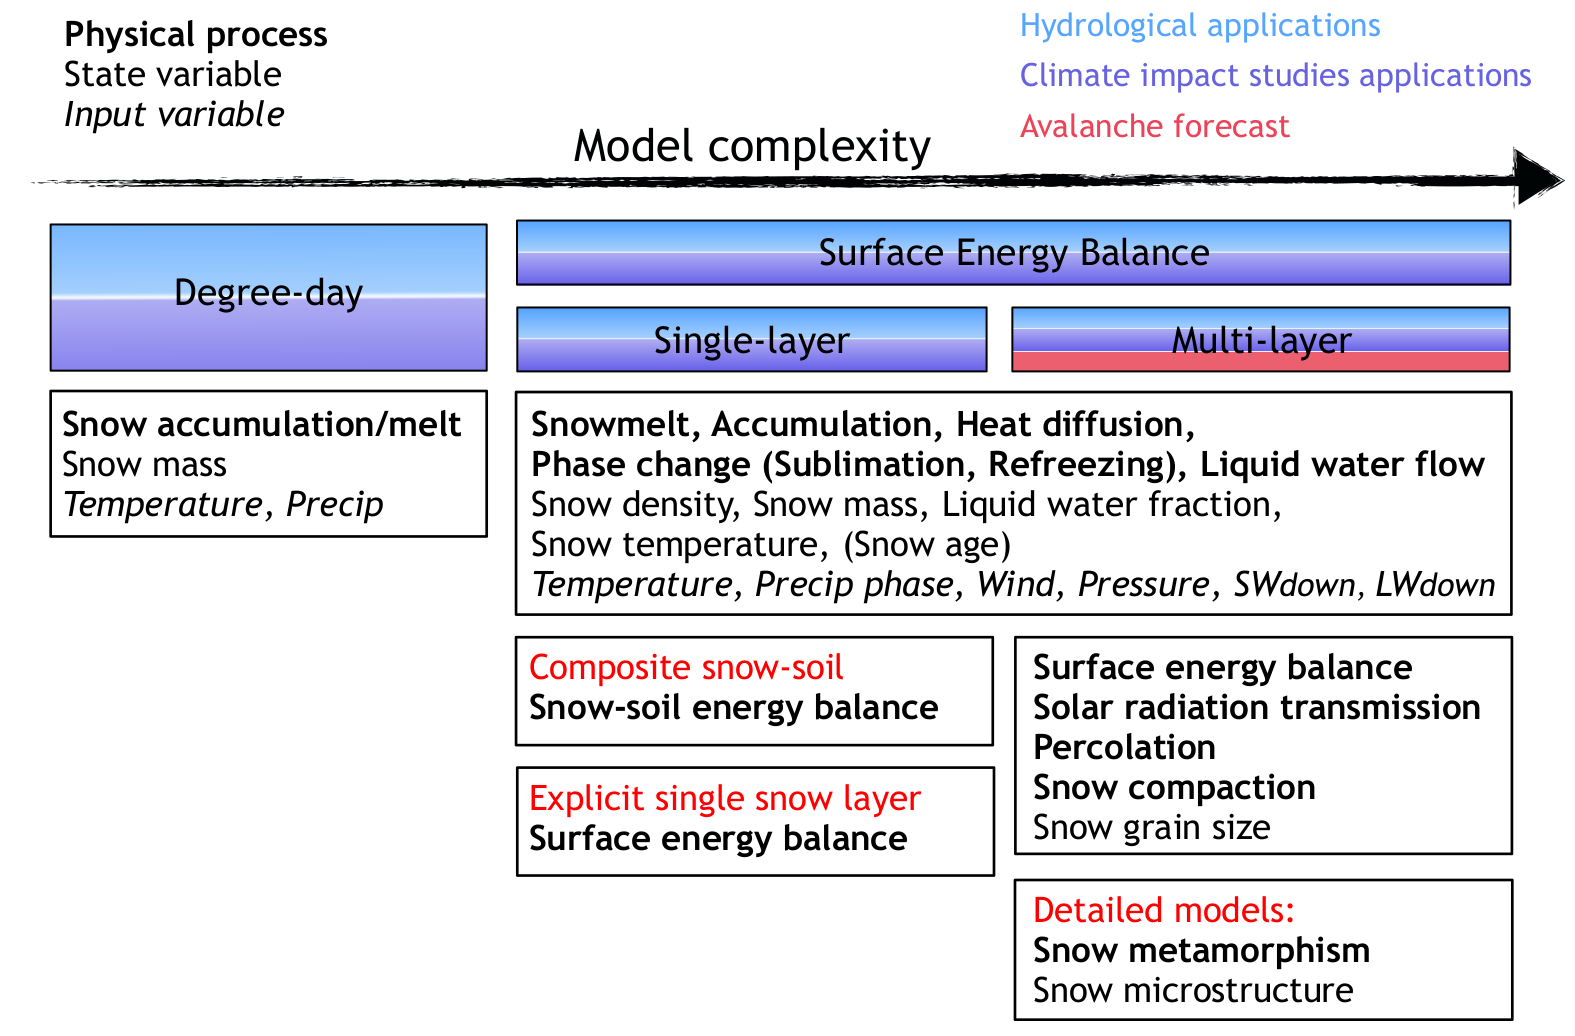
\includegraphics[scale=0.3]{Figures/Modelcomplexity_Article.png}
	\caption{Description of snow physical processes (bold), state variables (regular) and input variables (italic) required per category of snow models complexity for offline applications.}\label{Fig:Model_complexity}
\end{figure}


\section{Uncertainties and limits associated with snow models} 


Snowpack simulations are generally affected by several sources of uncertainties. First, the usefulness of snow model results depend, to a large extent, on the quality of the driving data. Meteorological forcing data from NWP model output contain errors impacting the snow simulations. This can be partly mitigated through data assimilation in atmospheric reanalysis such as ERA-Interim \citep{Dee_2011}, or at a more local scale with analysis systems assimilating observations of precipitation such as SAFRAN \citep{Durand_1993}. Meteorological input is often the dominating source of uncertainties of snow models outputs \citep{Fekete_2004,Bosilovich_2008,Raleigh_2015,Magnusson_2015}. The second source of uncertainties comes from the model itself (\textit{i.e.} the chosen parameters and simplifications in the description of the physical processes \citep{Essery_2013,Lafaysse_2017}). The uncertainties of snow simulations are also related to the sub-grid variability of the study area, especially in complex mountainous terrain, with features such as topography and slope as well as non-represented processes such as lateral redistribution of snow by wind contributing to the uncertainties. For models that includes snow and vegetation, the Snow-vegetation interactions are also a high source of energy balance uncertainties in snow models \citep{Boone_2017,Rutter_2009,Todt_2018}. The additional parameterisations (canopy model, snow interception, unloading, ...) make up for missing processes but also add uncertainties \citep{Mahat_2014}. Despite these additional uncertainties, they offer an improvement for forest areas \citep{Todt_2018}. The performance of a model and its evaluation can be established by ensemble simulations and model-intercomparison studies as described in the next sections.

%\subsection{Model errors}
%\subsubsection{Ensemble simulations}
\subsection{Ensemble simulations}

Ensemble approaches are increasingly used to estimate uncertainties pertaining to model output, helping to better describe the best configuration options and the mechanisms behind model performance. Ensemble simulations can be used to quantify the snow model errors due to the various contributions to the overall error distribution of the model. The latter is estimated through a number of simulations where each member uses slightly different initial conditions or physical options.  Multiple physics ensemble systems, such as JIM (JULES Investigation Model) \citep{Essery_2013,Raleigh_2015} or ESCROC \citep{Lafaysse_2017}, could be combined with ensemble NWP \citep{Molteni_1996,Descamps_2015,vernay2015} to represent uncertainties in both the snow model and in the meteorological forcings. However, ensemble models frequently remain under-dispersive leading to underestimate the model errors \citep{Vannitsem_2018}. When a model configuration is adjusted using observations, the performance of the model generally increases, what results in reduced errors and biases in the simulations \citep{Essery_2013}. The importance of using different sites for the evaluation of a model should be noted in order to avoid the danger of over-calibration at one site or one category of sites (\textit{e.g.} cold climate only, plain areas, ...) \citep{Essery_2013}.
The later study also demonstrates that there is not only one configuration of a model that provides the best simulation but an ensemble of configurations that yield the best results, however, with some configurations systematically providing inadequate results.
%It should be noted that the model have to be evaluated over different sites to avoid the danger of over-calibration at one site or one category of sites (\textit{e.g} cold climate only, plain areas) \citep{Essery_2013}.


\subsection{Model intercomparisons}

%Model-intercomparison excercises aim to better understand the difference between snow models that feature a wide range in complexity. Model-intercomparison projects such as ESM-SnowMIP \citep{Krinner_2018} include a large variety of models which are suitable for a range of climate conditions. 
Model intercomparison projects such as ESM-SnowMIP \citep{Krinner_2018} include a large variety of models suitable for a wide range of climate conditions. 
Physical snow processes in snow models are represented by different equations and parameterisations, and this leads to a spread of the predicted snowpack evolution under similar vegetation, soil and meteorological forcing conditions.  In this most recent model intercomparison ESM-SnowMIP project \citep{Krinner_2018}, the results show that for the 10 sites considered, the individual models which have the best performance with specific criteria such as SWE for all sites come from different models complexity. This illustrates that model complexity does not necessary explain the spread in performance. However, it is important to highlight that detailed snow models are more likely to be transferable in space and time, despite the challenging evaluation of the vertical profiles. %that the most detailed multi-layer snow models, such as Crocus, were among the best performing models. %Comparative studies have been carried out with the different versions of snow models of Météo-France \citep{Boone_2001,Vionnet_2012,Decharme_2016}. 

It is also known that snow model performance is much better at open sites than forest-sites \citep{Rutter_2009}. The inclusion of snow models into a land surface model improved the snow-vegetation interaction and SWE estimation \citep{Boone_2017}. Some studies have recently provided evidence that multi-layer canopy models \citep{Gouttevin_2015}, or those containing some sort of correction to bulk canopy models within LSMs are required to accurately represent the crucial longwave radiative interactions \citep{Todt_2018}.

The performance of a snow model generally differs during the accumulation and the ablation periods with often larger discrepancies during the melt period \citep{Etchevers_2004}. This induces a lower performance of the model during warm winters and overall warm sites due to a higher frequency of melt-events \citep{Etchevers_2004}. Models including prognostic snow density and albedo were shown to lead to better performances \citep{Essery_2013,Boone_2004}. The best simulations of snow mass and SWE correspond to model configurations options which retain melt water. The larger holding water capacity and refreezing results in an increase of the snowmelt runoff, leading to better discharge simulations \citep{Boone_2004} and better temporal evolution of SWE especially in high-latitudes \citep{Vionnet_2012,Decharme_2016}. %CL: Phrase ci dessous a supprimer? Cf Marie's comments
Additionally, snow depth is underestimated when configurations melt too early and is overestimated when snow density is underestimated \citep{Essery_2013}.

%V1:
%The prediction of snow accumulation and ablation differs from snow models, which leads to more significant difference during the snowmelt period \citep{Etchevers_2004}. This enhances a lower performance of the model during warmer winter and warmer sites due to higher frequency of melt-events \citep{Etchevers_2004}. Models including prognostic snow density and albedo were shown to lead to better performance \citep{Essery_2013,Boone_2004}. The best simulations in terms of snow mass use an hydrological option which retain melt water. Additionally, snow depth is underestimated when configurations melt too early and is overestimated when snow density is underestimated \citep{Essery_2013}. Model performance is much more consistent at open sites than forest-sites \citep{Rutter_2009}. In the most recent model intercomparison ESM-SnowMIP project \citep{Krinner_2018}, the results shows, for all sites and all years, that the most detailed multi-layer snow models, such as Crocus, was one of the best performing models. 
%Comparative studies have been carried out with different versions of snow models of Météo-France \citep{Boone_2001,Vionnet_2012,Decharme_2016}. The inclusion of the physical processes such as retention of liquid water in the multilayer model ISBA-ES resulted in an increase of the snowmelt runoff, which lead to better simulate SWE compared to the single snow layer of ISBA \citep{Boone_2001}. Due to a larger holding water capacity and condensation, Crocus simulates the largest SWE of the three models coupled to SURFEX, especially in high-latitudes. The integration of Crocus into ISBA (ISBA-Crocus), which represents snow-vegetation interaction, has lead to a better estimation of SWE \citep{Vionnet_2012}. 



\section{Combining observation and modelling: data assimilation}

\subsection{Concepts of data assimilation}

%Definir Objectif assimilation données:
Observations and numerical simulations represent two sources of information affected by uncertainties, that can be exploited simultaneously, thereby reducing the overall uncertainties of the output products. 
Data assimilation (DA) is the statistical and methodological approach that intents to achieve that goal. 
%SAM The principle of data assimilation (DA) relies on the combined use of models and observations to reduce such errors.  
DA was firstly used in weather forecasting systems to improve initial conditions of NWP and much latter for the estimation of parameter for model settings.
%SAM DA was firstly used in land-only and coupled land-atmosphere modelling systems to improve initial conditions of NWP and much latter for the estimation of parameter for model settings. %A series of observed quantities can be used to correct a forcing data or a physical state given by the model in order to obtain an optimal representation of the system under consideration.
A set of parameters or a physical state of the model can be corrected by a series of observed quantities to get a more accurate representation of the system under consideration. 
%SAM A forcing data or a physical state given by the model can be corrected by a series of observed quantities to get an optimal representation of the system under consideration. %Uncertainties pertaining to each observation quantity are used to weight their contribution in the data assimilation process. 
%SAM DA is characterised by a set of statistical methods aiming to improve the characteristics of a system by combining the information of models and observations.

\subsection{Data assimilation methods used in snow hydrology studies}


A wide range of DA methods exists which are more or less adapted to different applications depending on the limitations, the required level of complexity, the characteristics of the system, the frequency and the type of observations. 
%SAM A wide range of DA methods exist with different applications depending on the limitations, the required level of complexity, the characteristics of the system, the frequency and the type of observations. 
The DA methods easiest to implement have a sequential approach, where each set of observations is processed at a fixed time. Optimal interpolation (OI) is the most used in snow applications \citep{Helmert_2018}. However, OI is optimal only for nearly linear systems, and performs poorly with complex, highly nonlinear snow models. 
Other studies have used direct insertion methods which directly replace model states by observed values \citep{Rodell_2004,Liston_1999,Malik_2012} or Cressman interpolation \citep{Cressman_1959,Drusch_2004,Dee_2011}. The assimilation of snow observations in NWP are usually more simple than those used for the atmospheric component.


%The Kalman filter (KF) is an assimilation method that uses the calculation of the covariance error analysis and gain matrix to find the best analysed state. 
The Kalman filter (KF) is an assimilation method, that in addition to calculating an optimal analysed state, provides the associated errors. The standard version is optimal only for linear systems. To apply this method to weakly nonlinear systems, the Extended Kalman Filter (EKF) approach has been developed and uses a local linearisation of nonlinear systems using the tangent linearisation around a mean estimate and its associated covariance errors \citep{Miller_1994,Dong_2007}. This leads to an increase of computation time. 
For nonlinear systems, the DA estimate may encounter divergence issues with the EKF approach.
%SAM For nonlinear systems, the state of the model may encounter divergence issues with the EKF approach. 
In order to partly take into account the nonlinearity of the system, an ensemble-based approach has been developed: the ensemble KF (EnKF), that uses a Monte Carlo sampling of an ensemble of model states to propagate the error information \citep{Burgers_1998,Evensen_2000}. This approach loses accuracy for highly nonlinear systems and increases in computation cost when larger ensembles are needed. %This approach can also have a consequent computation cost for important ensemble size. %, which increases with the nonlinearity of a system and the matrix dimension.
The EnKF technique has been widely used in snow hydrology studies \citep[e.g.][]{Slater_2006,Andreadis_2006,Clark_2006,Su_2008,Thirel_2011,DeLannoy_2012,Huang_2017}. Another ensemble-based DA method is the particle filter with sequential importance resampling (PF-SIR; \citealp{gordon1993,Thirel_2011, Charrois_2016}). It uses an ensemble of simulations to represent the probability density function (PDF) of the system with no assumptions on the nature of the PDF. When an observation is available, each member of the ensemble, or particle, is weighted and then selected according to its distance to the observations. This method retains only the particles closest to the observations. These particle are then resampled according to their respective weights. This relatively simple method is particularly suitable for nonlinear system where the dynamics of the model is respected. Other approaches such as variational assimilation (1, 2 or 3D-Var) exist but have rarely been used in snow applications \citep{Dumont_2012} due to the necessity of an adjoint model and limited efficiency for non linear system.
A four-dimensional version, the 4D-Var, also exists but is more tricky to implement (\textit{e.g.} requiring an adjoint model) and has never been used in snow applications.
%Other approaches such as variational assimilation (\textit{e.g.} 4D-Var) used in NWP are more tricky to implement (\textit{e.g.} requiring an adjoint model) and are rarely used in snow application excepted few applications with the 1D-Var approach \citep{Dumont_2012,Phan_2014}. The variational methods consist in minimizing the cost function in order to reduce the distance between the observations and model states. % and are usually not used in snow applications. %More complex methods such as variational approaches (3D-Var, 4D-Var) used in NWP are not used in snow applications. The required adjoint model for this approach makes this method difficult to implement for complex detailed snow models. 

The comparison of the pros and cons of each category of sequential methods applied to snow observations and models have been summarised in Tab. \ref{tab:DA_method}. The DA scheme complexity increases with the finer resolution of the model and the longer prediction time horizon, as described in the Fig. 9 of \citet{Carrassi_2018}. The difficulties of OI, EKF and variational methods in dealing with nonlinearities make them generally not suited for complex nonlinear snow models. The capability of the EnKF to deal with large dimension error covariance matrices could be suitable for explicit snow models but this approach can also encounter issues related to its linearity assumption. To avoid nonlinearity issues, the particle filter is one of the most adequate data assimilation method for explicit detailed snow models. On the contrary to the other methods, particle filters are adequate to deal with the ensemble detailed snowpack simulations in which members may have a variable number of layers, i.e. variable dimension problem. However, in large dimension, this method has limitations when the resampling leads to very close particles which can lead to degeneracy. Because of its easy implementation and its ability to process nonlinear system, this technique has been used for a detailed multi-layer snow model and has shown promising results \citep[e.g.][]{Charrois_2016,Magnusson_2017}

\begin{table}
	%\centering
	\begin{center}
		\large
		\begin{tabular}{ l | c c c c c c}
			
			
			%			\diagbox[width=11em]{Characteristics}{ Methods}& \text{ OI }& \text{ PF } & \text{ PF-SIR } &\text{ EKF } &  \text{ EnKF } &  \text{ 3D-Var }  &  \text{ 4D-Var } \rule[2pt]{0pt}{10pt}\\			
			
			\text{}& \text{ OI }& \text{ PF-SIR } &\text{ EKF } &  \text{ EnKF } &  \text{1,2,3D-Var}  \rule[2pt]{0pt}{10pt}\\		
			\hline 
			\text{Sequential }& \text{$\checkmark$} & \text{$\checkmark$} &  \text{$\checkmark$} &  \text{$\checkmark$} & \text{$\checkmark$} \rule[0pt]{0pt}{15pt}\\		
			\text{Variational } & \text{} & \text{} & \text{} &  \text{} & \text{$\checkmark$} &\rule[0pt]{0pt}{15pt}\\			
			%		\text{Deterministic }& \text{$\checkmark$} & \text{} &  \text{} &  \text{$\checkmark$} &  \text{} & \text{$\checkmark$} &  \text{$\checkmark$}  \rule[0pt]{0pt}{15pt}\\
			\text{Ensemble } & \text{} &  \text{$\checkmark$} &  \text{} & \text{$\checkmark$} & \text{}  \rule[0pt]{0pt}{15pt}\\
			\hline
			%		\text{Gaussian}& \text{} & \text{} &  \text{} & \text{} &  \text{} & \text{} &  \text{}  \rule[0pt]{0pt}{15pt}\\
			\text{Easily implemented}& \text{$\color{green} \cmark$} & \text{$\color{green} \cmark$} & \text{$\color{orange} \cmark$} &  \text{$\color{orange} \cmark$} & \text{$\color{orange} \cmark$} \rule[0pt]{0pt}{15pt}\\			 
			\text{Calculation cost}& \text{$\color{green} \cmark$} & \text{$\color{orange} \cmark$} & \text{$\color{orange} \cmark$} &  \text{$\color{red} \xmark$} & \textbf{\color{orange} \cmark}  \rule[0pt]{0pt}{15pt}\\		
			\text{Nonlinearity capacity}& \text{$\color{red} \xmark$} &  \text{$\color{green} \cmark$} & \text{$\color{red} \xmark$} &  \text{$\color{orange} \cmark$} & \text{$\color{red} \xmark$} \rule[0pt]{0pt}{15pt}\\
			\text{High dimension capacity}& \text{$\color{orange} \cmark$} &  \text{$\color{red} \xmark$} & \text{$\color{red} \xmark$} &  \text{$\color{green} \cmark$} & \text{$\color{green} \cmark$}  \rule[0pt]{0pt}{15pt}\\		
			%			\text{Treshold issues}& \text{} & \text{} &  \text{} & \text{} &  \text{} & \text{$\color{red} \checkmark$} &  \text{$\color{red} \checkmark$}  \rule[0pt]{0pt}{15pt}\\	
			
		\end{tabular}	
	\end{center}
	\caption{Description of the different sequential data assimilation methods with their corresponding pros and cons applied to snow studies. A green check indicates a good adequacy of the method, an orange check a limited capacity and a red cross, strong limitations.}
	\label{tab:DA_method}	
\end{table}

%\begin{table}
%	%\centering
%	\begin{center}
%		\Large
%		\begin{tabular}{ l | c c c c c }
%			\text{}& \text{ OI }& \text{ PF-SIR } &\text{ EKF } &  \text{ EnKF }  \rule[2pt]{0pt}{10pt}\\		
%			\hline 
%			\text{Sequential }& \text{$\checkmark$} & \text{$\checkmark$} &  \text{$\checkmark$} &  \text{$\checkmark$} \rule[0pt]{0pt}{15pt}\\				
%			%		\text{Deterministic }& \text{$\checkmark$} & \text{} &  \text{} &  \text{$\checkmark$} &  \text{} & \text{$\checkmark$} &  \text{$\checkmark$}  \rule[0pt]{0pt}{15pt}\\
%			\text{Ensemble } & \text{} &  \text{$\checkmark$} &  \text{} & \text{$\checkmark$}   \rule[0pt]{0pt}{15pt}\\
%			\hline
%			%		\text{Gaussian}& \text{} & \text{} &  \text{} & \text{} &  \text{} & \text{} &  \text{}  \rule[0pt]{0pt}{15pt}\\
%			\text{Easily implemented}& \text{$\color{green} \cmark$} & \text{$\color{green} \cmark$} & \text{$\color{orange} \cmark$} &  \text{$\color{orange} \cmark$} \rule[0pt]{0pt}{15pt}\\			 
%			\text{Calculation cost}& \text{$\color{green} \cmark$} & \text{$\color{green} \cmark$} & \text{$\color{orange} \cmark$} &  \text{$\color{red} \xmark$}  \rule[0pt]{0pt}{15pt}\\		
%			\text{Nonlinearity capacity}& \text{$\color{red} \xmark$} &  \text{$\color{green} \cmark$} & \text{$\color{red} \xmark$} &  \text{$\color{orange} \cmark$}   \rule[0pt]{0pt}{15pt}\\
%			\text{High dimension capacity}& \text{$\color{orange} \cmark$} &  \text{$\color{red} \xmark$} & \text{$\color{red} \xmark$} &  \text{$\color{green} \cmark$} \rule[0pt]{0pt}{15pt}\\		
%			%			\text{Treshold issues}& \text{} & \text{} &  \text{} & \text{} &  \text{} & \text{$\color{red} \checkmark$} &  \text{$\color{red} \checkmark$}  \rule[0pt]{0pt}{15pt}\\	
%			
%		\end{tabular}	
%	\end{center}
%	\caption{Description of the different data assimilation methods with their corresponding pros and cons applied to snow studies. The capacity of a method is represented by a green check. The orange check corresponds to a restricted capacity. The red cross expresses the limitations of each method.}
%	\label{tab:DA_method}	
%\end{table}

%-Snow observation in DA

Lastly, batch smoother is another alternative DA approach that recently gained a lot of popularity in snow hydrology. Contrary to the DA methods detailed above that assimilate sequentially snow observations and only udpate the current state of the snowpack at the time of assimilation, batch smoothers take into account the entire history of the model trajectory and are more adequate to reanalysis problems. Such approach was introduce in snow hydrology among others by \citet{Margulis_2015} to produce SWE reanalysis based on SCA/SCF assimilation including in mountain areas. A detailed review of the application of such methodology to mountain snow hydrology is provided in \citet{Aalstad_2018}. 



\subsection{State of the art of snow observations used for data assimilation}

Due to the increase number of available observations, DA has been progressively integrated into land surface, hydrological and snow models during the last 20 years. Assimilation of snow observations have proven to be an essential tool to reduce the uncertainties for water resources. The first studies used simple conceptual hydrological and snow models integrating direct \textit{in situ} measurements, such as snow depth and SWE \citep{Day_1990, Carroll_1978}. Their integration has led to an improvement in the forecast of riverflow \citep{Day_1990} and snow cover runoff uncertainties were reduced by as much as  $40\,\%$ in a region where snow cover represents up to $80 \ \%$ of the water resource \citep{Carroll_1978}. Large-scale operational forecasts have started to assimilate snow data but using only \textit{in situ} snow measurements \citep{Brasnett_1999}. The assimilation of snow observations in an operational NWP system is usually made with observations of snow depth rather than SWE measurements due to the limited availability of such measurements \citep{Essery_2013}. The simultaneous assimilation of various snow variables has rarely been experimented, and has been tested only on local and offline simulations \citep{Piazzi_2018}. The latter study has shown that multivariate assimilation of snow surface temperature, surface albedo, SD and SWE has potential but raise new degeneracy challenges when using a particle filter. Detailed assimilation of \textit{in situ} observations of snow depth over all Switzerland at 250 m spatial resolution has been set up in \citet{Winstral_2019}. Such systems are highly efficient but rely of an extremely dense network of  \textit{in situ} observations (300 stations) that enables proper spatial propagation of the information through the input meteorological forcings \citep{Winstral_2019}. When the \textit{in situ} snow network is not dense enough, their assimilation remains limited in its ability to represent the spatial heterogeneity of the snow cover. For this reason, the combination of \textit{in situ} snow measurement with satellite observations is needed especially in regions with complex topography \citep{Magnusson_2015}. 

%The increased complexity of snow models has reinforced the need for new DA methods. In recent studies, an alternative approach to data assimilation has been investigated. This method consists in incorporating observations into multi-layer distributed snow models, where the ensemble members with observed snow depth have been evaluated over 300 sites in Switzerland . However, when the \textit{in situ} snow network is not dense enough, their assimilation remains limited in its ability to represent the spatial heterogeneity of the snow cover. For this reason, the combination of \textit{in situ} snow measurement with satellite observations is needed for better and more homogeneous results, especially in regions with complex topography \citep{Magnusson_2015}. 
% Ensemble members were evaluated using observed snow depths to ascertain potential biases at nearly 300 sites across Switzerland. The bias assessments were distributed to 38 independent sites and incorporated into the model. Tests were conducted over three winter seasons using two numerical weather prediction-based products with varying quality. 

%assimilation produits satellites optiques:
%SCA/SCF
The easiest method for integrating satellite observations in a snow model is the direct insertion method which is commonly used with optical images, and has been used extentively with MODIS SCA/SCF products \citep{Rodell_2004,Kumar_2008,Hall_2010,Fletcher_2012,Liu_2013}. %This method have proven an improvement for snow cover studies, including SWE estimations, in mid elevation compared to simulation without assimilation \citep{Rodell_2004,Kumar_2008,Arsenault_2013}. %The snow depletion curve (SDC) approach allows the estimations of SWE measurements from SCF informations \citep{Essery_2004}. %This approach is subject to significant uncertainties. 
This approach has resulted in an improvement of the simulated snow cover in comparison to simulations without assimilation, especially in the lowest (altitude) elevation bands and during the melting period \citep{Andreadis_2006,Arsenault_2013}. In contrast, the direct insertion method has shown a lower performance than with the EnKF assimilation  \citep{Arsenault_2013, Thirel_2011} and does not allow a backward correction of the simulation. Assimilation of optical SCA/SCF is also performed using particle filters approach \citep[e.g.][]{Thirel_2013, Baba_2018} leading to improved or similar performance that EnKF approaches. SWE reanalysis over long period have been produced using assimilation of SCA/SCF with different types of batch smoothers \citep[e.g.][]{Girotto_2014,Margulis_2015,Cortes_2017,Aalstad_2018}.
%In contrast, the performance of the EnKF remains better than the direct insertion for snowpack studies located at high elevation \citep{Arsenault_2013}. 

%ALBEDO
Optical satellite images have also been used to retrieve albedo data which plays an important role in the melting processes of the snowpack. Several studies have assimilated albedo products by using the direct insertion method, which shows improved estimations of snow depth, albedo and SWE  \citep{Malik_2012,Wang_2015}. Another approach is the assimilation of optical MODIS albedo products by using a 1D-Var method, which led to a $40 \%$ root-mean-square-error reduction in the mass balance of an alpine glacier \citep{Dumont_2012}. Snow cover simulations can be improved by combining different products such as an EnKF assimilation of SCF products and a direct insertion of albedo \citep{Xu_2016}. In addition, the assimilation of reflectance (spectral albedo) has been shown to further improve the simulated snowpack physical properties (\textit{e.g.} snow surface, \citealp{Charrois_2016}). The uncertainties related to the conversion of raw optical satellite imagery into snow products remain the main limitation of surface reflectance and albedo assimilation \citep{Zaitchik_2009,Hall_2010,DeLannoy_2012, Cluzet_2018}. The calculation of the observationnal errors is thus critical for the efficiency of the system.  Moreover, the assimilation of optical images is limited by the presence of clouds \citep{Hall_2007} which may be problematic in some mountainous regions \citep{Charrois_2016}. In contrast to EnKF, the use of particle filter over large domain may trigger degeneracy issues and does not provide a simple way forward to the spatial propagation of the assimilation from one pixel to the other. Localization methods are thus required \citep[e.g.][]{Farchi_2018}. Finally, \citet{Painter_2016} demonstrated that the assimilation of snow depth and albedo from airborn imagery in a physically-based snow model enable the retrieval of SWE maps at high resolution in moutain areas however restricted to the area covered by the planes. 

%RADAR:
A recent effort was made to assimilate the synthetic aperture radar (SAR) backscattered coefficients using a variational approach with a detailed multi-layer snow model \citep{Phan_2014}. This study showed promising results concerning the ability to correct density profiles over glaciers. However, large uncertainties on the observed backscattered signal make this approach difficult to use, and it requires an unbiased estimate of the observed data \citep{Veyssiere_2019}. Moreover, the radiative transfer model used to simulated the backscattered signal is more complex for RADAR data than for optical data generally leading to larger uncertainties \citep{Picard_2018, Helmert_2018}. 


%PASSIVE microwave:
%Data from passive microwave sensors can be used to provide data for assimilation schemes through either the use of raw brightness temperature or through retrieval algorithms to obtain a snow depth or SWE estimate, that can then be estimated from snow depth measurements and snow density \citep{Chang_1982}.
Numerous studies have been dedicated to the use of passive microwave observations. They rely either on the snow products generated from passive microwave sensors or on directly on raw brightness temperature\citep{Chang_1982}. The use of direct raw brightness temperature has been performed and show good results (where SWE estimations have relatively small uncertainties), especially during the accumulation period \citep{Durand_2007,DeLannoy_2012,Liu_2013,Liu_2015}. However, this method requires a radiative transfer model to simulate the brightness temperature that may contains a lot of uncertainties as for the RADAR signal. The highest uncertainties occur during the melting period, when the microwave signal is perturbed by liquid water contained in the snowpack. Limitations also arise from the bias in the retrieval algorithm \citep{Andreadis_2006,Dong_2007,Kumar_2008} as well as the uncertainties related to snow density, topography and interferences with vegetation \citep{DeLannoy_2012}. Several studies have combined the assimilation of SWE products with passive microwave AMSR-E observations and SCA/SCF products or reflectacne from optical MODIS images, which leads to better estimations of thin snowpack at medium latitude \citep{Durand_2007,Kumar_2008,DeLannoy_2012,Liu_2013,Fletcher_2012}. The EKF and EnKF method have been often used for the assimilation of SWE products from passive microwave satellites, such as AMSR-E and SMMR \citep{Andreadis_2006,Kumar_2008,DeLannoy_2012,Liu_2013}.
%The assimilation of snow products from passive microwave sensors can be done through the use of retrieval algorithm or directly with raw brightness temperature, where SWE products are estimated from snow depth measurements and snow density . The use of direct raw brightness temperature has been performed and show good results (where SWE estimations have relatively small uncertainties), especially during the accumulation period \citep{Durand_2007,DeLannoy_2012,Liu_2013,Liu_2015}. However, this method requires a radiative transfer model to simulate the brightness temperature. The highest uncertainties occur during the melting period, when the microwave signal is perturbed by liquid water contained in the snowpack. The performances of the assimilation of SWE products remain limited by the coarse resolution of the satellite data (around 20 km). Limitations also arise from the bias in the retrieval algorithm \citep{Andreadis_2006,Dong_2007,Kumar_2008} as well as the uncertainties related to snow density, topography and interferences with vegetation \citep{DeLannoy_2012}. Several studies have combined the assimilation of SWE products with passive microwave AMSR-E observations and SCA/SCF products with optical MODIS images, which leads to better estimations of thin snowpack at medium latitude \citep{Kumar_2008,DeLannoy_2012,Liu_2013,Fletcher_2012}. The EKF and EnKF method have been often used for the assimilation of SWE products from passive microwave satellites, such as AMSR-E and SMMR \citep{Andreadis_2006,Kumar_2008,DeLannoy_2012,Liu_2013}. %The performance of the assimilation of SWE is directly linked to the correction of the algorithm bias \citep{Liu_2013,Liu_2015}. 
A recent study has assimilated passive microwave AMSR-2 satellite observations in a detailed snow model using the particle filter, which was shown to reduce the bias of SWE estimation by up to $71 \ \%$ over flat areas \citep{Larue_2018}. However, the coarse spatial resolution of passive microwave satellites limits the application for snow products over mountain regions. %Despite its limitations, recent studies attempt to retrieve passive microwave information for deep mountainous snowpack. These studies 
Recent studies have been however carried out by assimilating airborne observations of high-resolution passive microwave imagery for SWE estimations for deep mountainous snowpack \citep{Li_2017,Kim_2019}. The latter study demonstrated that very accurate SWE simulations are obtained with the use of a detailed snow model and with a particle filter approach, whereas the SWE estimation from passive microwave were severely degraded when a three-layer snow model or the Kalman filter analysis scheme were used \citep{Kim_2019}.

%V1:
%Despite its limitations, a recent study has attempt to use passive microwave with a high resolution model to allows to downscale the coarse microwave measurements by using an Ensemble Batch Smoother (an alternative of the EnKF method) \citep{Li_2017}. A more recent study have applied this latter method to mountain terrains by using the particle filter approach, showing that there is a hope for estimating SWE for deep mountainous snowpack using passive microwave measurements \citep{Kim_2019}.
%V2:
%The recent study of \citet{Kim_2019} highlights the need to use a detailed snow model and with a particle filter approach, since the evaluation of SWE estimation from passive microwave signal proved to be degraded when a three-layer snow model or the Kalman filter analysis scheme were used.

%Parag. de conclu:
%Dire que beaucoup d'études ont utilisé l'assimilation de données pour app. neige
%Assimilation of \textit{in situ} and satellite observations has been largely used in snow applications and usually led to a reduction of the uncertainties related to the snow models. DA has been studied with different type of satellites associated to varying performances. Most DA studies in mountain areas have used optical satellites due to their high spatial resolution. More recent studies proceed to the assimilation of microwave satellites despite their associated difficulties (\textit{\textit{e.g.} retrieval algorithm, spatial resolution}). To date, SWE estimations can be mostly retrieved from passive microwave radiance observations. The coarse resolution of spaceborne passive microwave limits their use to flat areas. More recently, DA of airborne passive microwave satellite has proven to be useful for mountain regions provided the use of a high resolution detailed snow model for deep snowpacks. %Note that, until now, there has been no attempt of combining various satellite observations of snow (\textit{e.g.} optical and microwave) in the same data assimilation procedure. This challenge is likely to meet similar difficulties as in the multivariate \textit{in situ} assimilation framework of \citet{Piazzi_2018}.
%Dire que possible d'utiliser uw si modèle de neige détaillé avec données aéroporté (pour meilleur res.)




\section{Summary and recommendations}

%1)Necessite données:
%Snow on the ground is a crucial component of the energy exchanges on the climate system and of the hydrological cycle. 
The monitoring of snow is essential to predict water resources and snow-related natural hazards. This monitoring can be partially achieved by using \textit{in situ} and satellite observations. \textit{In situ} snow measurements provide critical data for characterising the snow cover at a given location. These measurements do not provide information on spatial heterogeneity. Issues related to the representativeness and scarcity of point-scale \textit{in situ} data makes the use of satellite observations unavoidable for monitoring snow spatial variability. Yet, \textit{In situ} snow measurements remain essential for the evaluation and the calibration of snow models, as well as the evaluation of satellite-based products and development of DA algorithms in controlled environments. For satellites and \textit{in situ} observations, the choice of observation type depends on the required information and the purpose of the study. Depending on the desired applications, the required spatial and temporal resolution also can lead a developer to use different satellites observations. A high spatial resolution is a necessary prerequisite for monitoring the snow cover in mountain areas due to the complex topography and the subsequent significant spatial heterogeneity of the snow cover properties. 

%2)Detailler Av/Inc chaque données satellites:
The snow properties to which a remote sensor is sensitive vary with the satellite frequencies and type (optical, thermal infrared and microwave). Monoscopic and stereoscopic optical sensors are limited to cloud-free days during the daytime. Monoscopic optical satellites provide multi-spectral images in the visible and near infrared wavelength with a relatively high spatial resolution (20 - 500 m). They generally provide snow cover area (SCA) and snow cover fraction (SCF) information, surface properties such as albedo, light absorbing particles of the snow and snow microstructure, but they cannot directly measure water equivalent of snow cover (SWE). Stereoscopic optical satellites provide snow depth information at very high spatial resolution (0.5 - 2 m), but this technique contains substantial uncertainties ($\pm$ 50 cm), only operates on demand for a reduced set of observation dates, and it is generally restricted to small areas. The long-wave energy radiation from passive microwave has the advantage to provide information under any weather condition (clouds, rain and night), that can be used as a predictor for snow depth and SWE. The coarse resolution of passive microwave satellites (20-40 km) is, however, not sufficient for mountain areas and its use is limited to non-complex terrain, such as flat areas. %Passive microwave has been shown to be powerful to allow estimation of snow properties such as SWE over large relatively flat areas despite its large uncertainties. % \citep{Larue_2018}. 
For mountain applications, the complex topography requires the use of high spatial resolution satellite data, such as optical and SAR observations. %The latter emit their own signal and detect the backscattered signal, thereby providing images of snow extent with a high spatial resolution (10 - 20 m). 
However, disentangling the contribution of the different snowpack properties (density, stratigraphy, ....) to the SAR signal remains extremely challenging without \textit{a priori} knowledge of the structure and the physical properties of the snowpack.


%3)Justifier choix modèle de neige:

%The representation of physical processes of snow in models is essential to monitor and predict the evolution of the snowpack. A large variety of snow models exist with different levels of complexity of the representation of the snow physical processes.
In addition to observations, the use of snow models is required to monitor the evolution of the snowpack. The physical characteristics and processes are represented in snow models with varying levels of complexity. The choice of the model complexity is determined by applications as well as the spatial and temporal extent of the application. It is further constrained by the computational capabilities and the availability of meteorological forcings, where the number of meteorological inputs is higher for the more complex schemes, such as Surface Energy Balance models. The increase of computing performance has permitted the more widespread use of detailed multi-layer snow models which represent the physical properties of the snowpack. Their use is associated with uncertainties related to the chosen parameterisation, the initial conditions, and the input meteorological data. The most recent snow model intercomparison studies have shown that % detailed explicit multi-layer snow models generally lead to the best performance. 
the best performance comes from different model complexity, including a detailed explicit multi-layer snow model. Despite these advances in predicting SWE and snow characteristics only based on numerial simulations, many uncertainties persist. This leads to combine the use of snow models and snow observations.

%4)Donner méthode d'assimilation à utiliser:


%%%%% begin MARIE

The assimilation of \textit{in situ} and satellite observations of snow has been increasingly used in snow applications and usually led to a reduction of the uncertainties related to the snow simulations. Data assimilation of \textit{in situ} observations of snow depth is one of the most efficient methods to provide SWE estimates when the observation network is dense enough which is the case only for some rare regions of the Earth. Satellite data are thus the most natural source of information to constrain snowpack simulations uncertainties in regions where \textit{in situ} observations are too sparse. The satellite data most commonly used in DA for SWE estimation are SCA/SCF from optical satellites and passive microwave data, the spatial resolution of the latter being too coarse to be relevant for mountain areas. SCA/SCF assimilation with batch smoothers can provide relatively accurate SWE reconstruction in mountain areas. However, ensemble assimilation of raw satellite signals from SAR or optical sensors is one of the most promising way to really improve SWE prediction at high resolution. Though promising results have been shown, several issues need to be tackle to built highly efficient prediction systems. First, the assimilation of such data requires an \textit{a priori} knowledge of the vertical structure of the snowpack which fosters the use of detailed snowpack models and accurate observation operators that includes both the terrain effects in link with the rugged topography and the electromagnectic interactions within the snowpack. Second, such system are highly non-linear which plays in favor of DA methods such as batch smoothers, particle filters and to a minor extent EnKF. Third, the determination of the observation errors remains crucial for such system. And, finally, the methodology used for the spatialization of the assimilation procedure over large areas is also not perfectly bounded especially in the case of particle filters. Data assimilation methodology issues in case of combined assimilation of various types of observations are also to be foreseen. Such prediction system would enable not only accurate probablistic SWE prediction but also a better knowledge of the snowpack physical properties, that is a prerequisite for instance for avalanche hazards forecasting. New satellite observations such as snow depth from stereo-imagery \citep{Margulis_2019} or high resolution surface temperature would most likely largely improve the reliability of such prediction systems.  





%%%%% end MARIE



%DA was first used with only \textit{in situ} snow observations. The scarcity of these measurements led to the combination of such observations with satellite data in locations where \textit{in situ} observations are not dense enough. The assimilation of satellite observations often requires an observation operator using multi-layered snow information. For this reason, snow data assimilation often requires detailed multi-layer snow models. %These models are thus essential to properly assimilate satellite signal and to determine the physical properties of the snowpack. 
%The use of such models for the assimilation of satellite signal leads to a better representation of the snow microstructure and stratigraphy, thus contributing to improve the performance of DA. The representation of physical processes in these snow models are described by nonlinear equations. One of the optimal method consists in the use of ensemble assimilation technique that is suitable for nonlinear systems. For such systems, the most suitable DA techniques are the EnKF and the particle filter methods, despite possible divergence issues. %The particle filter approach have usually shown better results compared to the EnKF. 
%Most studies using a detailed multi-layer snow models have used these two ensemble methods with promising results. Several studies have shown that assimilation of optical and microwave satellite data leads to a better performance by using the particle filter than the EnKF. Recent studies have shown encouraging results on using SWE assimilation with microwave observations. The assimilation of passive microwave has proven to be more efficient when using direct raw luminance than a retrieval algorithm to assimilate SWE estimations. This can be explained by the biases induced by the retrieval algorithms. However, the assimilation of raw data requires a radiative transfer model to simulate brightness temperature. The assimilation of passive-microwave satellites with a detailed snow model enhances better estimations of thin snowpack over flat areas. However, the coarse resolution of these satellite limits their use to non-complex mountainous terrains. Since mountainous complex terrains require a high resolution satellite observations, to date, their use is limited to optical satellites or radar. Due to the high uncertainties conducted by the backscatter of the radar signal, the assimilation of snow products in mountain regions is usually performed using optical satellites observations to retrieve SCA/SCF and albedo informations.

%In the future, we recommend the use of a detailed snow model and an ensemble DA approach such as particle filter showing promising results. TO DO...
%%%%%%%%%%%%%%%%%%%%%%%%%%%%%%%%
%%%%%%%%%%%%%%%%%%%%%%%%%%%%%%%%%

%Importance suivi manteau neigeux avalanche
%besoin de reduire incertitude
%assim données
%besoin de modèle de neige detaillé

%V1: In summary, the optimal method of snow data assimilation is to use a detailed multi-layer snow model with an ensemble assimilation technique that is suitable for nonlinear equations, such as the particle filter approach. The estimation of SWE products can be conducted by using passive microwave satellite for large plains areas. For applications in mountain areas, the complex terrains require the choice of high resolution satellite observations combined with \textit{in situ} measurements.

%V3: In summary, the monitoring of the snowpack is essential for various applications (\textit{e.g.} water resources, avalanches forecasting). The representation of snow in models is also essential to better represent the energy exchanges in the soil-biosphere-snow-atmosphere interactions. \textit{In situ} and satellites observations are crucial for the evaluation of models. DA techniques use the combination of models and observations in order to reduce their associated uncertainties. The choice of satellites vary according to the applications as well as the spatial and temporal resolution. The required DA technique depends of the model complexity. [...]

%V2:
%In summary, choosing the appropriate method depends on the type of model and observation used, and on the target application of modelling system. The use of a detailed multi-layer snow model for the assimilation of satellite signal leads to a better representation of the physical processes of snow, thus contributing to limit the uncertainties. One of the optimal methods consists in an ensemble assimilation technique that is suitable for nonlinear systems. The assimilation method can also be chosen according to its ease of use and implementation, such as the particle filter approach. The use of remote sensed data (satellite or terrestrial) is crucial for large scale studies, especially for regions with complex topography. The choice of the type of satellite varies with the required spatial and temporal resolution of the study. For applications in mountain areas, the complex terrains require the choice of high resolution satellite observations, such as optical satellites or radar. Due to the high uncertainties conducted by the backscatter of the radar signal, the assimilation of snow products in mountain regions is usually performed using optical satellites observations.
%The performance of data assimilation and related problems also depends on the type of observed data used. The assimilation of optical satellites has better performance by using the particle filter than the EnKF. With passive microwave satellites, the assimilation of raw luminance has proven to be more efficient than the assimilation of SWE estimation through retrieval algorithms due to the high associated bias \citep{Durand_2009,DeLannoy_2012}. The assimilation of raw data requires a radiative model to simulate brightness temperature. The coarse resolution of passive microwave limits its use to non-complex terrain, such as flat areas. The assimilation of radar data is rarely used due to the high uncertainties of the observed data, as well as the complexity to simulate the backscattered radar signal and its significant associated uncertainties. For snow mountain applications, the complex topography requires the use of high spatial resolution such as optical and SAR satellites observations.






%%%%%%%%%%%%%%%%%%%
%%%%% THE END %%%%%

\section{Nomenclature}









\section*{Conflict of Interest Statement}
The authors declare that the research was conducted in the absence of any commercial or financial relationships that could be construed as a potential conflict of interest.

\section*{Author Contributions}
C.L. wrote the initial draft of the paper. All authors contributed to the writing-review $\&$ editing of the final written version

\section*{Funding}
The CNRM/CEN and IGE are part of Labex OSUG@2020. The research was partly funded by CNES, MAGELLIUM and by the ANR program ANR-16-CE01-0006 EBONI.

A COMPLETER.

\section*{Abbreviations}

The following abbreviations are used in this manuscript:\\
	
\noindent 
\begin{tabular}{@{}ll}
		SCA & Snow Cover Area\\
		SCF & Snow Cover Fraction\\
		DA & Data Assimilation\\
		EKF & Extended Kalman Filter\\
		EnKF & Ensemble Kalman Filter\\
		ESB & European Snow Booklet\\
		IFS & Integrated Forecast System\\
		KF & Kalman Filter\\
		NDSI & Normalized Difference Snow Index\\
		NWP & Numerical Weather Prediction\\
		OI & Optical Interpolation\\
		PDF & Probability Density Function\\
		SAR & Synthetic Aperture Radar\\
		SEB & Surface Energy Balance\\
		SnowMIP & Snow Model Intercomparison Project\\
		SPICE & Solid Precipitation Intercomparison Experiment\\
		SWE & Water Equivalent of Snow cover\\
		WMO & World Meteorological Organisation
\end{tabular}

\bibliographystyle{frontiersinSCNS_ENG_HUMS} % for Science, Engineering and Humanities and Social Sciences articles, for Humanities and Social Sciences articles please include page numbers in the in-text citations
%\bibliographystyle{frontiersinHLTH&FPHY} % for Health, Physics and Mathematics articles
%\bibliography{test}
%\externalbibliography{yes}
\bibliography{BiblioSWE.bib}

%%% Make sure to upload the bib file along with the tex file and PDF
%%% Please see the test.bib file for some examples of references



\end{document}
